\chapter{JADE e JASON}

\section{JADE}

\subsection{FIPA}

\dfn{FIPA}{
  Consorzio per la standardizzazione di sistemi ad agenti. Il suo obiettivo era quello di promuovere tecnologie interoperabili: sistemi di agenti intelligenti che lavorano insieme.
}

\qs{}{Cosa rientrà nelle competenze di FIPA?}

\begin{itemize}
  \item Gestione del ciclo di vita di un agente. 
  \item Come trasportare un messaggio. 
  \item La struttura di un messaggio. 
  \item Protocolli di interazione tra agenti. 
  \item Ontologie e sicurezza.
\end{itemize}

\nt{Gli agenti sono al di fuori degli obiettivi di FIPA.}

\paragraph{Caratteristiche che vengono assunte per gli agenti:}

\begin{itemize}
  \item Autonomi. 
  \item Reattivi. 
  \item Proattivi. 
  \item Goal-driven. 
  \item Sociali. 
  \item Adattivi. 
  \item Cognitivi.
\end{itemize}

\begin{figure}[!h]
    \centering
    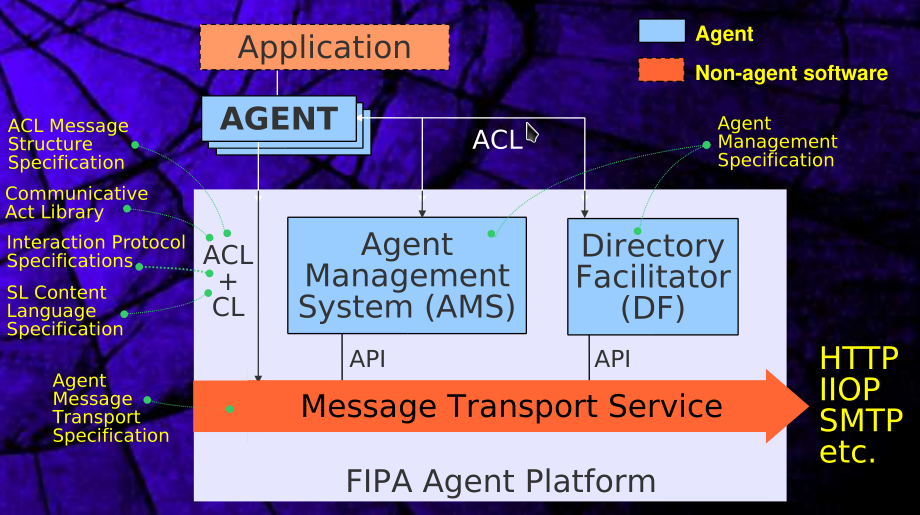
\includegraphics[scale=0.35]{05/FIPA.png}
  \caption{Piattaforma FIPA per agenti.}
\end{figure}

\cor{Agent Management}{
  Gli agenti hanno una descrizione di sé stessi e dei servizi che vengono offerti. L'Agent Management sistem è a sua volta un agente con cui si interagisce con scambi di messaggi. In jade si può accedere così oppure accedere direttamente agli oggetti Java.
}

\begin{figure}[!h]
    \centering
    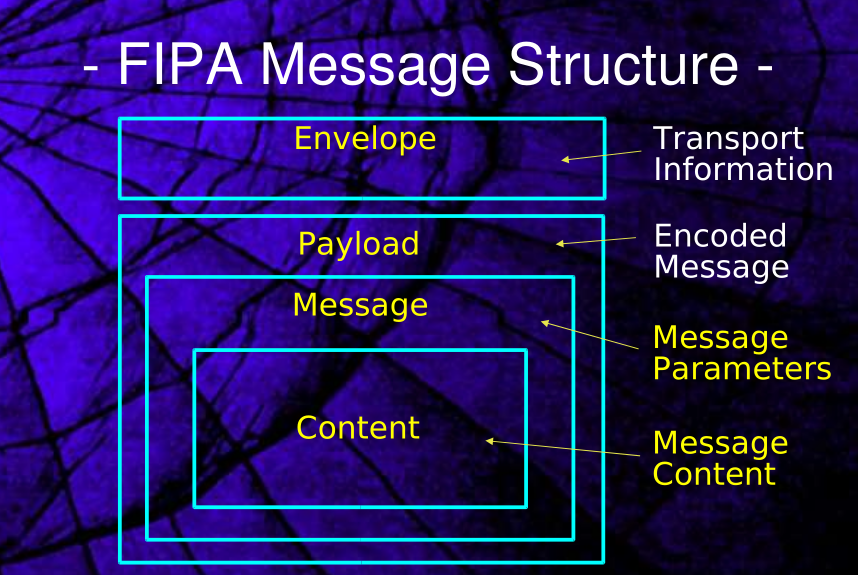
\includegraphics[scale=0.35]{05/messaggi.png}
  \caption{Specifica per i messaggi.}
\end{figure}

\subsection{Introduzione a JADE}

\qs{}{Che cos'è JADE?}

\paragraph{Risposta:} JADE è la piattaforma, all'interno del consorzio FIPA, che implementa lo standard sopra citato. Si presenta come codice Java puro. Offre una serie di librerie per agenti e un runtime envinronment per gli agenti creati. L'obiettivo è quello di "nascondere" FIPA al programmatore. 

\begin{figure}[!h]
    \centering
    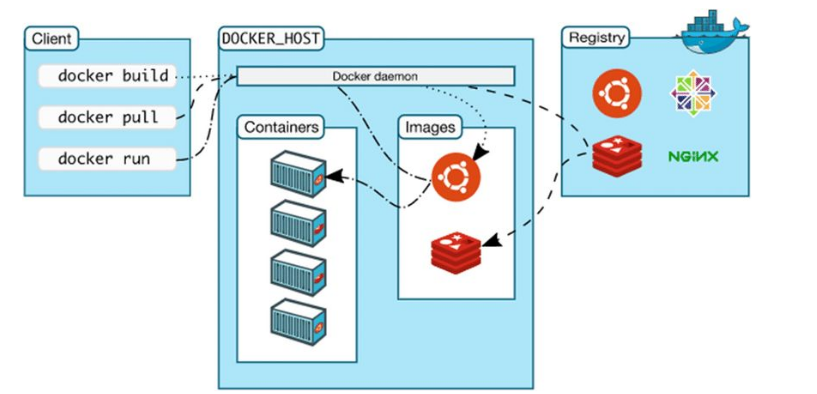
\includegraphics[scale=0.45]{05/arch.png}
  \caption{Modello architetturale di JADE.}
\end{figure}

\paragraph{Caratteristiche importanti:}

\begin{itemize}
  \item \fancyglitter{HalloWorld Agent:}
    \begin{itemize}
      \item Un tipo di agente è creato estendendo \texttt{jade.core.Agent} e ridefinendo il metodo \texttt{setup()}. 
      \item Ogni agente è identificato da un AID (nome univoco e qualche indirizzo).
      \item A ogni agente è assegnato uno e un solo thread (per evitare deadlock).
    \end{itemize}
  \item \fancyglitter{Local names, GUID and addresses:}
    \begin{itemize}
      \item Il nome completo di un agente deve essere globalmente unico. 
      \item In una singola piattaforma JADE ci si riferisce agli agenti solamente mediante il loro nome. 
      \item È possibile creare AID. 
      \item Si possono passare argomenti agli agenti.
    \end{itemize}
  \item \fancyglitter{Terminazione:}
    \begin{itemize}
      \item Un agente termina quando è chiamato il metodo \texttt{doDelete()}. Questo metodo non cancella all'istante, ma segnala che l'agente deve essere eliminato (solo dopo aver completato la \texttt{setup()}. 
      \item Nella terminazione è chiamato il metodo \texttt{takeDown()} per fare operazioni di clean-up.
    \end{itemize}
\end{itemize}

\dfn{Classe Behaviour}{
Il lavoro si un agente è eseguito dalle sue "behaviours". Per far sì che un agente esegua un task è sufficiente definire una behaviour e aggiungerla all'agente. 
}

\paragraph{Ogni behaviour deve implementare:}

\begin{itemize}
  \item \texttt{void action():} cosa la behaviour fa. 
  \item \texttt{boolean done():} quando la behaviour finisce.
\end{itemize}

\nt{Un agente può eseguire più behaviours in parallelo, il loro scheduling è cooperativo e tutti avvengono nello stesso thread java.}

\begin{figure}[!h]
    \centering
    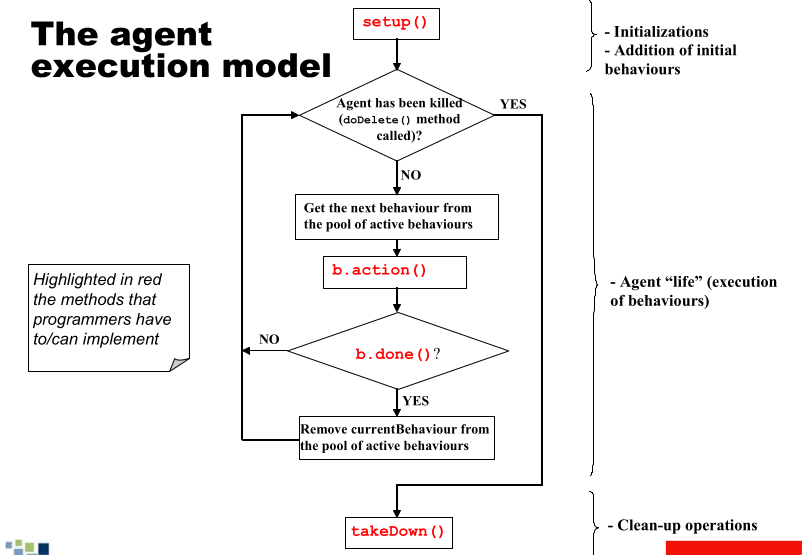
\includegraphics[scale=0.5]{05/exec.png}
  \caption{Modello di esecuzione di un agente.}
\end{figure}

\paragraph{Tipi di behaviour:}

\begin{itemize}
  \item \fancyglitter{One shot:}
    \begin{itemize}
      \item La loro \texttt{action()} viene eseguita solo una volta. 
      \item \texttt{done()} restituisce sempre true (non si deve reimplementare).
    \end{itemize}
  \item \fancyglitter{Cyclic:}
    \begin{itemize}
      \item Non si completano mai, \texttt{action()} effettua sempre le stesse operazioni. 
      \item \texttt{done()} restituisce sempre false (non si deve reimplementare).
    \end{itemize}
  \item \fancyglitter{Complex:}
    \begin{itemize}
      \item Hanno uno stato (e.g. DFA) e a seconda di esso svolgono operazioni differenti. 
      \item Completano quando una data condizione diventa vera.
    \end{itemize}
\end{itemize}

\paragraph{Altri tipi:}

\begin{itemize}
  \item \fancyglitter{WakerBehaviour:}
    \begin{itemize}
      \item Al posto di \texttt{action()} e \texttt{done()} si deve ridefinire \texttt{onWake()} che verrà eseguito dopo un certo timeout. 
      \item Subito dopo l'esecuzione il behaviour è completato.
    \end{itemize}
  \item \fancyglitter{TickerBehaviour:}
    \begin{itemize}
      \item Al posto di \texttt{action()} e \texttt{done()} si deve ridefinire \texttt{onTick()} che verrà eseguito periodicamente.
      \item L'esecuzione va avanti all'infinito o finché non viene invocato \texttt{stop()}. 
      \item Solitamente si usa per aggiungere periodicamente delle behaviours.
    \end{itemize}
\end{itemize}

\paragraph{Other shits on behaviours:}

\begin{itemize}
  \item \texttt{onStart():} invocato prima della prima esecuzione di \texttt{action()}. Sono operazioni che devono essere eseguite prima di ogni behaviour.
  \item \texttt{onEnd():} invocato dopo che \texttt{done()} restituisce true. Sono operazioni che devono essere eseguite alla fine di ogni behaviour.
  \item \texttt{removeBehaviour():} well, prova a indovinare cosa fa... RIMUOVE LA FUCKING BEHAVIOUR DAL POOL DI UN AGENTE\footnote{Non chiama \texttt{onEnd}.}. 
  \item Quando il pool di behaviours attive di un agente è vuoto esso entra in IDLE a il suo thread va in sleep.
\end{itemize}

\subsection{Comunicazione tra Agenti}

\dfn{Modello di Comunicazione}{
  Il modello di comunicazione è basato sul passaggio asincrono di messaggi. I messaggi sono definiti dal linguaggio ACL (FIPA).
}

\begin{figure}[!h]
    \centering
    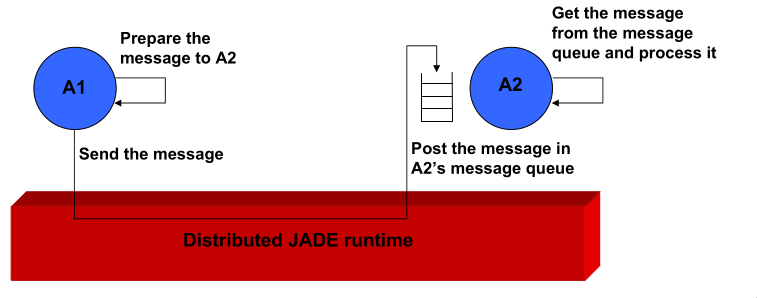
\includegraphics[scale=0.65]{05/mess.png}
  \caption{Modello di comunicazione.}
\end{figure}

\paragraph{I messaggi:}

\begin{itemize}
  \item Invio: inviare i messaggi è la creazione di un messaggio ACL e l'invio del messaggio tramite \text{send(ACLMessage)}.
  \item Ricezione: per leggere i messaggi si usa \texttt{receive()}.
\end{itemize}

\paragraph{Bloccare una behaviour mentre si aspetta per un messaggio:}

\begin{itemize}
  \item Il metodo \texttt{block()} non blocca il thread, ma sposta il behaviour dal pool di comportamenti attivi in un pool di comportamenti bloccati. 
  \item Non è una chiamata bloccante. 
  \item Tutte le behaviours vengono riattivate quando arriva un nuovo messaggio.
\end{itemize}

\paragraph{Leggere selettivamente una coda di messaggi:}

\begin{itemize}
  \item \texttt{receive()} restituisce il primo messaggio nella coda di messaggi e lo rimuove. 
  \item Se ci sono più behaviours che aspettano un messaggio una può rubare il messaggio a un'altra behaviour interessata. 
      \item Per evitare questo è possibile leggere solo certi tipi di messaggi con certe caratteristiche.
\end{itemize}

\paragraph{Ricevere un messaggio in "modalità bloccante":}

\begin{itemize}
  \item Gli agenti hanno anche un metodo \texttt{blockingReceive()} che restituisce quando c'è un messaggio nella coda di messaggi.
  \item Questa è una chiamata bloccante, per cui nessuna altra behaviour può eseguire finché la behaviour che ha invocato il metodo non ha ricevuto un messaggio.
\end{itemize}

\dfn{Pagine Gialle}{
Un servizio che consente agli agenti di pubblicare uno o più servizi che forniscono in modo che gli altri agenti possano trovarli.
}

\nt{In JADE ci si può accedere come oggetto remoto o interagendo come fosse un agente con messaggi ACL (modalità imposta da FIPA).}

\begin{figure}[!h]
    \centering
    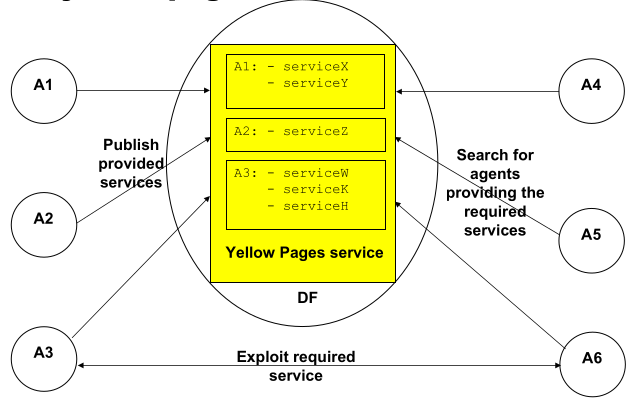
\includegraphics[scale=0.6]{05/yellow.png}
  \caption{Servizio di pagine gialle.}
\end{figure}

\pagebreak

\subsection{Protocolli di Interazione}

\dfn{Protocolli di Interazione}{
  Hanno un insieme di tipi di messaggio (INFORM, REQUEST, PROPOSE, \dots) che consentono lo scambio di specifiche sequenze predefinite di messaggi durante una conversazione.
}

\begin{figure}[!h]
    \centering
    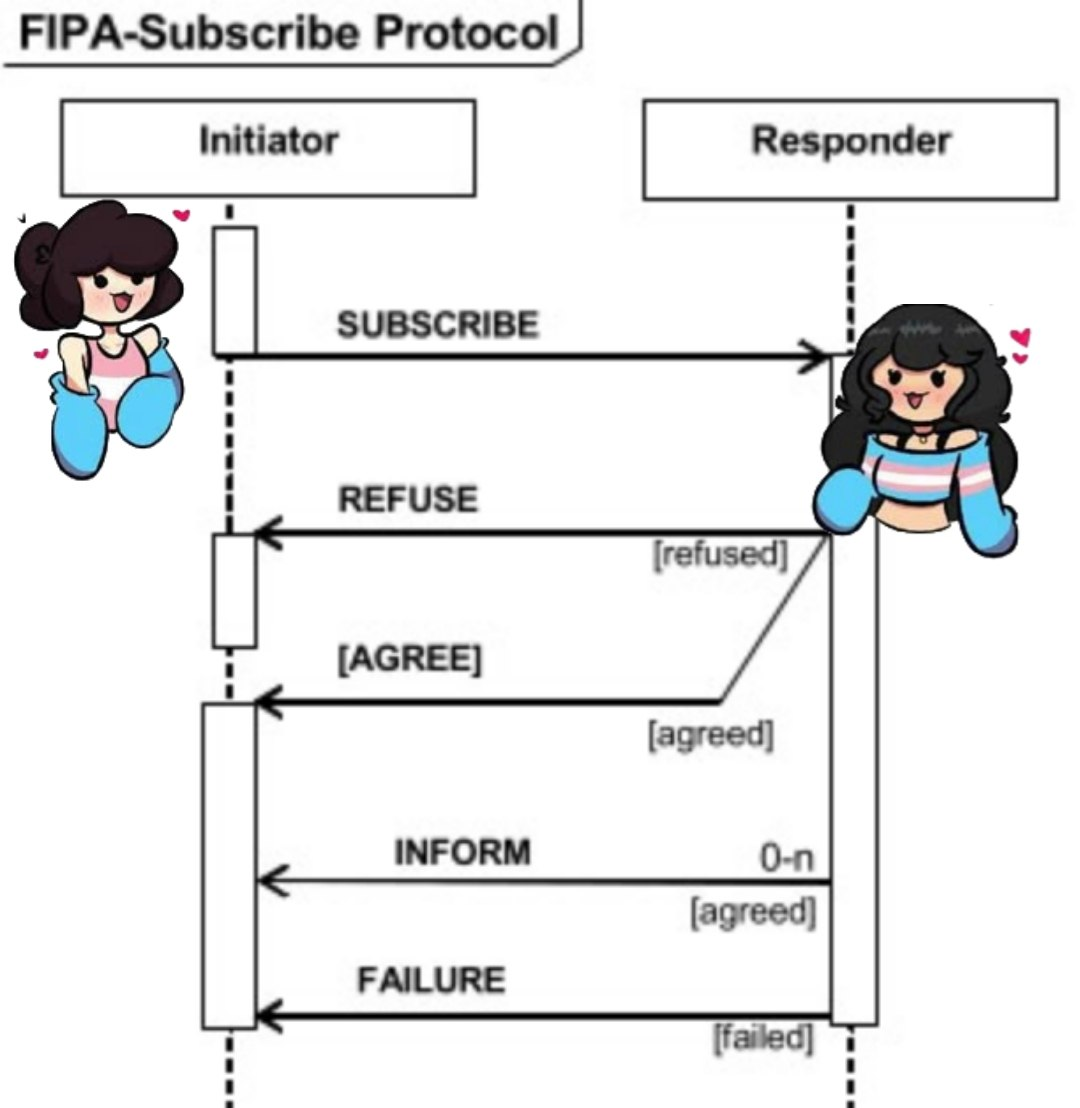
\includegraphics[scale=0.35]{05/FIPA_SUB.jpg}
  \caption{FIPA Protocol.}
\end{figure}

\paragraph{Alcuni protocolli comuni sono già presenti:}

\begin{itemize}
  \item Request. 
  \item Contract-net. 
  \item Subscribe.
\end{itemize}

\paragraph{Essi garantiscono:}

\begin{itemize}
  \item Che il flusso di messaggi sia compliant con il protocollo. 
  \item Che se è presente un timeout esso sia corretto.
\end{itemize}

\section{JASON}

\subsection{Introduzione}

\dfn{AgentSpeak}{
  Un linguaggio di programmazione per agenti che si propone di colmare il gap tra specifica teorica e implementazione di un agente.
}

\nt{JASON è un'implementazione di AgentSpeak, scritta in java.}

\clm{}{}{
  \begin{itemize}
    \item Gli agenti BDI vengono trattati sotto due punti di vista:
      \begin{itemize}
        \item Specifica teorica. 
        \item Implementazione.
      \end{itemize}
    \item Le implementazioni esistenti usano strutture dati per rappresentare \fancyglitter{belief}, \fancyglitter{desires} e \fancyglitter{intentions}.
    \item JASON è un'estensione della programmazione logica (e.g. prolog).
  \end{itemize}
}

\paragraph{Agenti BDI:}

\begin{itemize}
  \item Sistemi collocati in un ambiente dinamico, che muta nel tempo. 
  \item Sistemi in grado di percepire informazioni provenienti dall'ambiente. 
  \item Sistemi in grado di compiere delle azioni sulla base dei propri stati mentali, in particolare:
    \begin{itemize}
      \item Belief: cattura le informazioni. 
      \item Desire: cattura le motivazioni. 
      \item Intention: catture le decisioni.
    \end{itemize}
\end{itemize}

\subsection{AgentSpeak(L)}

\qs{}{Ma com'è fatto AgentSpeak(L)?}

\begin{itemize}
  \item Si parte da un BDI. 
  \item Il sistema è PRS (Procedural Reasoning System) e dMARS (Distribuited Multi-Agent Reasoning System). 
  \item Si basa sulla logica del primordine con eventi e azioni. 
  \item A differenza di BDI si vanno a scrivere programmi. 
  \item Dettaglio dell'agente: 
    \begin{itemize}
      \item Current belief: modello di sé stesso, dell'ambiente e degli altri agenti. 
      \item Desires: stati che l'agente vuole raggiungere. 
      \item Intentions: adozione di programmi per soddisfare certi stimoli.
    \end{itemize}
\end{itemize}

\paragraph{Il linguaggio AgentSpeak(L):}

\begin{itemize}
  \item Testuale. 
  \item Possiede belief (predicati), piani, azioni, intentions, eventi e goals. 
  \item Piani:
    \begin{itemize}
      \item Context-sensitive. 
      \item Possono essere invocati dall'utente. 
      \item Decomposizione gerarchica dei goals.
      \item Simili alle clausole di prolog.
    \end{itemize}
  \item Usa un alfabeto composto da variabili, costanti, simboli funzionali, simboli predicativi, simboli di azione, connettivi, quantificatori e punteggiatura. 
  \item I connettivi sono: 
    \begin{itemize}
      \item $\&$: congiunzione. 
      \item not: negazione. 
      \item $\leftarrow$: implicazione. 
      \item !: achievement goal. 
      \item ?: test goal. 
      \item ;: sequenza.
    \end{itemize}
\end{itemize}

\dfn{Belief}{
  Siano $b(t)$ e $c(s)$ belief atoms, allora $b(t) \& c(s)$ e not $b(t)$ sono beliefs.
}

\cor{Belief Atom}{
  Sia $b$ un simbolo predicativo e siano $t_1,\dots,t_n$ termini, allora: $b(t_1,\dots,t_n)$ è un belief atom e si scrive anche $b(t)$.
}

\nt{Un belief atom e la sua negazione sono detti belief literal. Se un belief atom è ground (senza variabili libere) si chiama belief base.}

\dfn{Goal}{
  Sia $g$ un simbolo predicativo e siano $t_1,\dots,t_n$ termini, allora: !$g(t_1,\dots,t_n)$ è un achievement goal, ?$g(t_1,\dots,t_n)$ è un test goal.
}

\paragraph{Triggering event:}

\begin{itemize}
  \item Quando un agente acquisisce un nuovo goal oppure nota una modifica nell'ambiente può far scattare aggiunte/cancellazioni di goals o beliefs. 
  \item L'aggiunta è rappresentata dall'operatore +. 
  \item La rimozione dall'operatore -.
\end{itemize}

\dfn{Azione}{
  Sia $a$ un simbolo di azione e siano $t_1,\dots,t_n$ termini, allora $a(t_1,\dots,t_n)$ è un'azione.
}

\paragraph{Piano:}

\begin{itemize}
  \item Un piano specifica il modo in cui un agente potrebbe raggiungere un determinato obiettivo. 
  \item Un Triggering event specifica perché il piano è stato attivato. 
  \item Il context specifica quali beliefs dovrebbero essere soddisfatti nel set di credenze dell'agente quando il piano scatta. 
  \item Il body è una sequenza di goals o azioni e specifica:
    \begin{itemize}
      \item I goals. 
      \item Le azioni.
    \end{itemize}
  \item true rappresenta un componente vuoto.
\end{itemize} 

\dfn{Piano}{
  Siano:
  \begin{itemize}
    \item $e$ un triggering event. 
    \item $b_1,\dots,b_m$ belief literals. 
    \item $h_1,\dots,h_n$ goals o azioni. 
  \end{itemize}

  allora
  $$e:b_1\&\dots\&b_m \leftarrow h_1,\dots,h_n$$
  è un piano.
}

\nt{La parte sinistra della freccia è detta \fancyglitter{head}, la parte destra della freccia è detta \fancyglitter{body} (un body vuoto è true). La parte a destra dei ":", nell'head, è il contesto.}

\subsection{Semantica Operazionale}

\paragraph{Un agente può essere visto come costituito da:}

\begin{itemize}
  \item Un insieme di beliefs $B$. 
  \item Un insieme di piani $P$. 
  \item Un insieme di intentions $I$. 
  \item Un insieme di eventi $E$. 
  \item Un insieme di azioni $A$. 
  \item Un insieme di funzioni di selezione: $S_\epsilon, S_O, S_I$.
\end{itemize}

\paragraph{Progetto di un agente:}

\begin{itemize}
  \item Il progettista specifica un agente scrivendo:
    \begin{itemize}
      \item Un insieme di base belief. 
      \item Un insieme di piani.
    \end{itemize}
  \item Si definiscono:
    \begin{itemize}
      \item Un insieme di fatti. 
      \item Un insieme di regole.
    \end{itemize}
\end{itemize}

\paragraph{Reasoning Cycle:}

\begin{enumerate}
  \item Viene generato un triggering event quando un agente nota una modifica dell'ambiente circostante (esterno) o quando un utente esterno chiede all'agente di raggiungere un goal (interno). 
  \item Gli eventi vengono inseriti in un set $E$. 
  \item Viene applicata la funzione di revisione dei beliefs:
    \begin{itemize}
      \item $S_\epsilon$ seleziona in $E$ un evento $E_0$ da processare. 
      \item $E_0$ viene rimosso da $E$ e viene usato per unificare con i triggering events dei piani $P$. 
      \item I piani che unificano sono detti \fancyglitter{piani rilevanti} e il loro unificatore si chiama \fancyglitter{unificatore rilevante}.
    \end{itemize}
  \item L'unificatore rilevante è applicato al contesto dei piani rilevanti. Una \fancyglitter{correct answer substitution} è ottenuta dal contesto. 
  \item Per alcuni piani le condizioni dei contesti risultano essere conseguenze logiche del set dei base beliefs $B$. Questi piani sono detti \fancyglitter{piani applicabili} mediante un \fancyglitter{unificatore applicabile} (derivato dalla composizione tra correct answer substitution e unificatore rilevante).
  \item Dato un evento $E_0$ diversi piani risultano applicabili, per cui la funzione di selezione $S_0$ sceglie uno di questi ($P_0$). Applicando l'unificatore applicabile a $P_0$ si ottiene l'\fancyglitter{intended means} in risposta al triggering event. Ogni intention è uno stack di piani parzialmente istanziati (intention frames). 
  \item A seconda del tipo di evento:
    \begin{itemize}
      \item Esterno: l'intended means è usato per creare una nuova intention che viene aggiunta a $I$. 
      \item Interno: l'intended means è inserito in cima all'intention esistente che ha fatto scattare l'evento.
    \end{itemize}
  \item Quando l'agente esegue un intention:
    \begin{itemize}
      \item Eseguire un achievement goal equivale a generare un evento interno per aggiungere il goal alla corrente intention. 
      \item Eseguire un test goal equivale a trovare una sostituzione per il goal che lo renda una conseguenza logica dei base belief. Se viene trovata una sostituzione il test goal è rimosso. 
      \item Eseguire un'azione equivale ad aggiungerla al set di azioni $A$ e rimuoverla dal corpo.
    \end{itemize}
  \item L'agente torna a valutare il set degli eventi $E$ e il ciclo ricomincia fino a quando il set $E$ è vuoto o non è possibile eseguire altre intentions. 
\end{enumerate}

\begin{figure}[!h]
    \centering
    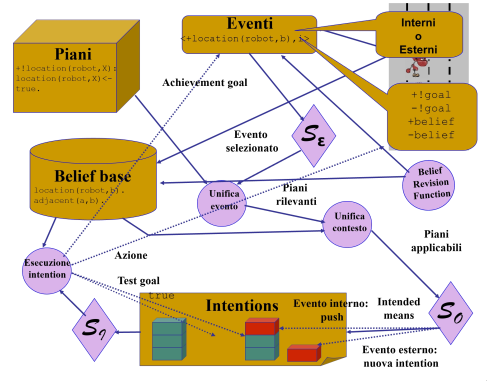
\includegraphics[scale=0.5]{05/reasoning.png}
  \caption{Reasoning Cycle.}
\end{figure}

\dfn{Intention}{
  $I$ è l'insieme delle intentions. Ogni intention è uno stack di piani parzialmente istanziati, ossia piani dove alcune variabili sono state istanziate. Un'intention è denotata come: $[p_1|p_2|\dots|p_z]$
}

\nt{Caso particolare (true intention): $[$ +!true: true $\leftarrow$ true$]$}

\dfn{Evento}{
  L'insieme $E$ è l'insieme degli eventi. Ogni evento è una coppia $\langle e, i \rangle$ dove:
  \begin{itemize}
    \item $e$ è un triggering event. 
    \item $i$ è una intention.
  \end{itemize}
}

\nt{Se $i$ è la true intention T, l'evento è esterno, altrimenti è interno.}

\paragraph{Ancora sui piani:}

\begin{itemize}
  \item Scelto un evento $\langle d, i \rangle$ dal set $E$, il triggering event $d$ viene unificato con i triggering event di tutti i piani contenuti nel set $P$. 
  \item Il \fancyglitter{most general unifier}\footnote{Che schifo IALAB.} (mgu) che unifica i due eventi è detto relevant unifier. 
  \item L'intention $i$ può essere:
    \begin{itemize}
      \item La true intention. 
      \item Un'intention esistente che ha generato l'evento.
    \end{itemize}
\end{itemize}

\clm{}{}{
  \begin{itemize}
    \item Un piano rilvante è anche applicabile se esiste una sostituzione che composta con l'unificatore rilevante e applicata al contesto fa sì che quest'ultimo risulti una conseguenza logica dei base beliefs $B$.
    \item La condizione del contesto di un piano rilevante deve essere conseguenza logica di $B$ affinché il piano sia applicabile.
  \end{itemize}
}

\subsection{JASON: Un'Implementazione di AgentSpeak(L)}





